 \documentclass[12pt,letterpaper]{article}
\usepackage[utf8]{inputenc}
\usepackage[spanish, es-tabla]{babel}
\usepackage[version=3]{mhchem}
\usepackage[journal=jacs]{chemstyle}
\usepackage{amsmath}
\usepackage{amsfonts}
\usepackage{amssymb}
\usepackage{makeidx}
\usepackage{xcolor}
\usepackage{verbatim}
\usepackage[stable]{footmisc}
\usepackage[section]{placeins}
%Paquetes necesarios para tablas
\usepackage{longtable}
\usepackage{array}
\usepackage{xtab}
\usepackage{multirow}
\usepackage{colortab}
%Paquete para el manejo de las unidades
\usepackage{siunitx}
\sisetup{mode=text, output-decimal-marker = {,}, per-mode = symbol, qualifier-mode = phrase, qualifier-phrase = { de }, list-units = brackets, range-units = brackets, range-phrase = --}
\DeclareSIUnit[number-unit-product = \;] \atmosphere{atm}
\DeclareSIUnit[number-unit-product = \;] \pound{lb}
\DeclareSIUnit[number-unit-product = \;] \inch{"}
\DeclareSIUnit[number-unit-product = \;] \foot{ft}
\DeclareSIUnit[number-unit-product = \;] \yard{yd}
\DeclareSIUnit[number-unit-product = \;] \mile{mi}
\DeclareSIUnit[number-unit-product = \;] \pint{pt}
\DeclareSIUnit[number-unit-product = \;] \quart{qt}
\DeclareSIUnit[number-unit-product = \;] \flounce{fl-oz}
\DeclareSIUnit[number-unit-product = \;] \ounce{oz}
\DeclareSIUnit[number-unit-product = \;] \degreeFahrenheit{\SIUnitSymbolDegree F}
\DeclareSIUnit[number-unit-product = \;] \degreeRankine{\SIUnitSymbolDegree R}
\DeclareSIUnit[number-unit-product = \;] \usgallon{galón}
\DeclareSIUnit[number-unit-product = \;] \uma{uma}
\DeclareSIUnit[number-unit-product = \;] \ppm{ppm}
\DeclareSIUnit[number-unit-product = \;] \eqg{eq-g}
\DeclareSIUnit[number-unit-product = \;] \normal{\eqg\per\liter\of{solución}}
\DeclareSIUnit[number-unit-product = \;] \molal{\mole\per\kilo\gram\of{solvente}}
\usepackage{cancel}
%Paquetes necesarios para imágenes, pies de página, etc.
\usepackage{graphicx}
\usepackage{lmodern}
\usepackage{fancyhdr}
\usepackage[left=4cm,right=2cm,top=3cm,bottom=3cm]{geometry}

%Instrucción para evitar la indentación
%\setlength\parindent{0pt}
%Paquete para incluir la bibliografía
%\usepackage[backend=bibtex,style=chem-acs,biblabel=dot]{biblatex}
%\addbibresource{references.bib}

%Formato del título de las secciones

\usepackage{titlesec}
\usepackage{enumitem}
\titleformat*{\section}{\bfseries\large}
\titleformat*{\subsection}{\bfseries\normalsize}

%Creación del ambiente anexos
\usepackage{float}
\floatstyle{plaintop}
\newfloat{anexo}{thp}{anx}
\floatname{anexo}{Anexo}
\restylefloat{anexo}
\restylefloat{figure}

%Modificación del formato de los captions
\usepackage[margin=10pt,labelfont=bf]{caption}

%Paquete para incluir comentarios
\usepackage{todonotes}

%Paquete para incluir hipervínculos
\usepackage[colorlinks=true, 
            linkcolor = blue,
            urlcolor  = blue,
            citecolor = black,
            anchorcolor = blue]{hyperref}


%%%%%%%%%%%%%%%%%%%%%%
%Inicio del documento%
%%%%%%%%%%%%%%%%%%%%%%

\begin{document}

\title{Control Automático\\Proyecto 2}

\author{Jorge Rojas Meza\\201006018\\Julio Viveroe Hernández\\}
\date{\today}
\maketitle
\section{Introducción}
Se analizó en el laboratorio cierto sistema y se construyó su respuesta en frecuencia (Diagrama de Bode) en lazo abierto y es la única información disponible para el diseño de los reguladores. Para el desarrollo de este proyecto 2, es obligatorio utilizar Scilab. Además deberá de generar un informe utilizando Latex en la plataforma \textit{Overleaf}.

\section{Problema}

Considere el Diagrama de Bode ed la función de transferencia en lazo cerrado directo que se presenta en la Figura 1.\\
\begin{figure}
  \centering
    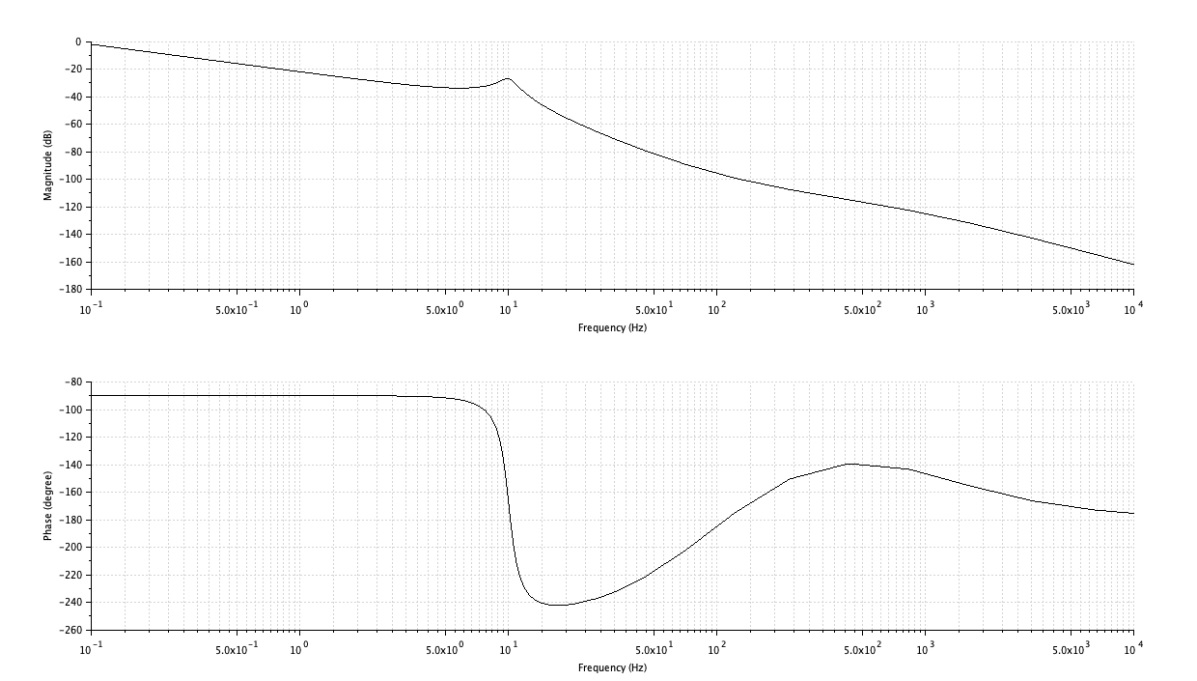
\includegraphics[width=0.6\textwidth]{Figura1.jpg}
  \caption{Respuesta en Frecuencia del Sistema en análisis.}
  \label{fig:ejemplo}
\end{figure}

Se desean diseñar diferentes sistemas de control que se adapten y mejoren el comportamiento de lazo cerrado del mismo y que cumplan con las siguientes especificaciones:

\begin{itemize}
    \item Error cero cuando la referencia es un escalón.
    \item Error menor al 10$\%$ cuando la referencia es una rampa.
    \item Margen de fase mayor o igual a 60$^\circ$, de tal forma que al aproximar el sistema en lazo cerrado a un sistema de segundo orden se obtenga un spbreimpulso no mayor al 20$\%$.
\end{itemize}

El diagrama presentado en la Figura 2 permite visualizar un acercamiento al pico máximo de resonancia del sistema y su respectiva frecuencia.\\

\begin{figure}
  \centering
    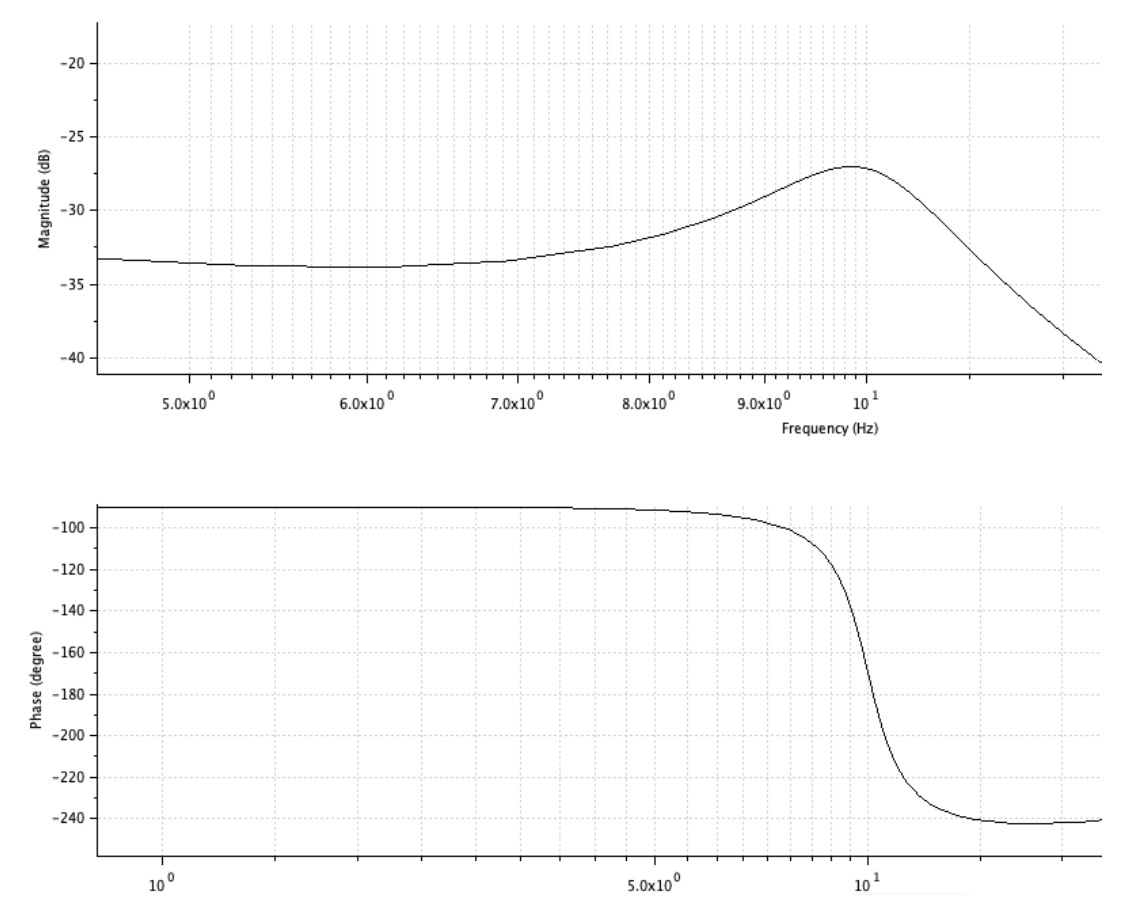
\includegraphics[width=0.6\textwidth]{Fig2.jpg}
  \caption{Zoom del pico de resonancia máxima y su frecuencia.}
  \label{fig:ejemplo}
\end{figure}


A continuación se presentan algunas relaciones de interés para el desarrollo de los diseños:

\begin{equation}
    \xi = \frac{MF}{100}
\end{equation}

\begin{equation}
    M_r = \frac{1}{2\xi\sqrt{1-\xi^2}}
\end{equation}

\begin{equation}
    \omega_r = \omega_n \sqrt{1-2\xi^2}
\end{equation}

\begin{equation}
    M_p = \exp^\frac{-\pi\xi}{\sqrt{1-\xi2}}
\end{equation}


\begin{equation}
    e_{ss}= \lim_{s \to 0} \frac{sR(s)}{1+G(s)H(s)}
\end{equation}


Donde $\xi$ es el factor de amortiguamiento, MF es el Margen de Fase, $M_r$ el pico máximo de ganancia a la frecuencia de resonancia $\omega_r$, $M_p$ el sobreimpulso y $e_{ss}$ el error de estado estacionario que depende de la entrada R(s). Se puede además estimar de forma aproximada el tiempo de levantamiento como t_r $\approx$ 1.8/$\omega_n$. Además se recuerda que el ancho de banda se determina en la frecuencia de -3dB.

\section{Cuestionamientos}
1. Asumiendo que H(s) = 1. Encuentre la función de transferencia de lazo abierto a partirde los diagramas de Bode proporcionados.


\nocite{*}
\bibliographystyle{ieeetr}
\bibliography{main.bib}
\end{document}




